\documentclass[aspectratio=169]{../latex_main/tntbeamer}  % you can pass all options of the beamer class, e.g., 'handout' or 'aspectratio=43'
\usepackage{dsfont}
\usepackage{bm}
\usepackage[english]{babel}
\usepackage[T1]{fontenc}
%\usepackage[utf8]{inputenc}
\usepackage{graphicx}
\graphicspath{ {./figures/} }
\usepackage{algorithm}
\usepackage[ruled,vlined,algo2e,linesnumbered]{algorithm2e}
\usepackage{hyperref}
\usepackage{booktabs}
\usepackage{mathtools}

\usepackage{amsmath,amssymb}

\DeclareMathOperator*{\argmax}{arg\,max}
\DeclareMathOperator*{\argmin}{arg\,min}

\usepackage{amsbsy}
\newcommand{\vect}[1]{\bm{#1}}
%\newcommand{\vect}[1]{\boldsymbol{#1}}

\usepackage{pgfplots}
\pgfplotsset{compat=1.16}
\usepackage{tikz}
\usetikzlibrary{trees} 
\usetikzlibrary{shapes.geometric}
\usetikzlibrary{positioning,shapes,shadows,arrows,calc,mindmap}
\usetikzlibrary{positioning,fadings,through}
\usetikzlibrary{decorations.pathreplacing}
\usetikzlibrary{intersections}
\pgfdeclarelayer{background}
\pgfdeclarelayer{foreground}
\pgfsetlayers{background,main,foreground}
\tikzstyle{activity}=[rectangle, draw=black, rounded corners, text centered, text width=8em]
\tikzstyle{data}=[rectangle, draw=black, text centered, text width=8em]
\tikzstyle{myarrow}=[->, thick, draw=black]

% Define the layers to draw the diagram
\pgfdeclarelayer{background}
\pgfdeclarelayer{foreground}
\pgfsetlayers{background,main,foreground}

% Requires XeLaTeX or LuaLaTeX
%\usepackage{unicode-math}

\usepackage{fontspec}
%\setsansfont{Arial}
\setsansfont{RotisSansSerifStd}[ 
Path=../latex_main/fonts/,
Extension = .otf,
UprightFont = *-Regular,  % or *-Light
BoldFont = *-ExtraBold,  % or *-Bold
ItalicFont = *-Italic
]
\setmonofont{Cascadia Mono}[
Scale=0.8
]

% scale factor adapted; mathrm font added (Benjamin Spitschan @TNT, 2021-06-01)
%\setmathfont[Scale=1.05]{Libertinus Math}
%\setmathrm[Scale=1.05]{Libertinus Math}

% other available math fonts are (not exhaustive)
% Latin Modern Math
% XITS Math
% Libertinus Math
% Asana Math
% Fira Math
% TeX Gyre Pagella Math
% TeX Gyre Bonum Math
% TeX Gyre Schola Math
% TeX Gyre Termes Math

% Literature References
\newcommand{\lit}[2]{\href{#2}{\footnotesize\color{black!60}[#1]}}

%%% Beamer Customization
%----------------------------------------------------------------------
% (Don't) Show sections in frame header. Options: 'sections', 'sections light', empty
\setbeamertemplate{headline}{empty}

% Add header logo for normal frames
\setheaderimage{
	% 
\includegraphics[height=\logoheight]{figures/TNT_darkv4.pdf}
	
\includegraphics[height=\logoheight]{../latex_main/figures/luh_logo_rgb_0_80_155.pdf}
	% 
\includegraphics[height=\logoheight]{figures/logo_tntluh.pdf}
}

% Header logo for title page
\settitleheaderimage{
	% 
\includegraphics[height=\logoheight]{figures/TNT_darkv4.pdf}
	
\includegraphics[height=\logoheight]{../latex_main/figures/luh_logo_rgb_0_80_155.pdf}
	% 
\includegraphics[height=\logoheight]{figures/logo_tntluh.pdf}
}

% Title page: tntdefault 
\setbeamertemplate{title page}[tntdefault]  % or luhstyle
% Add optional title image here
%\addtitlepageimagedefault{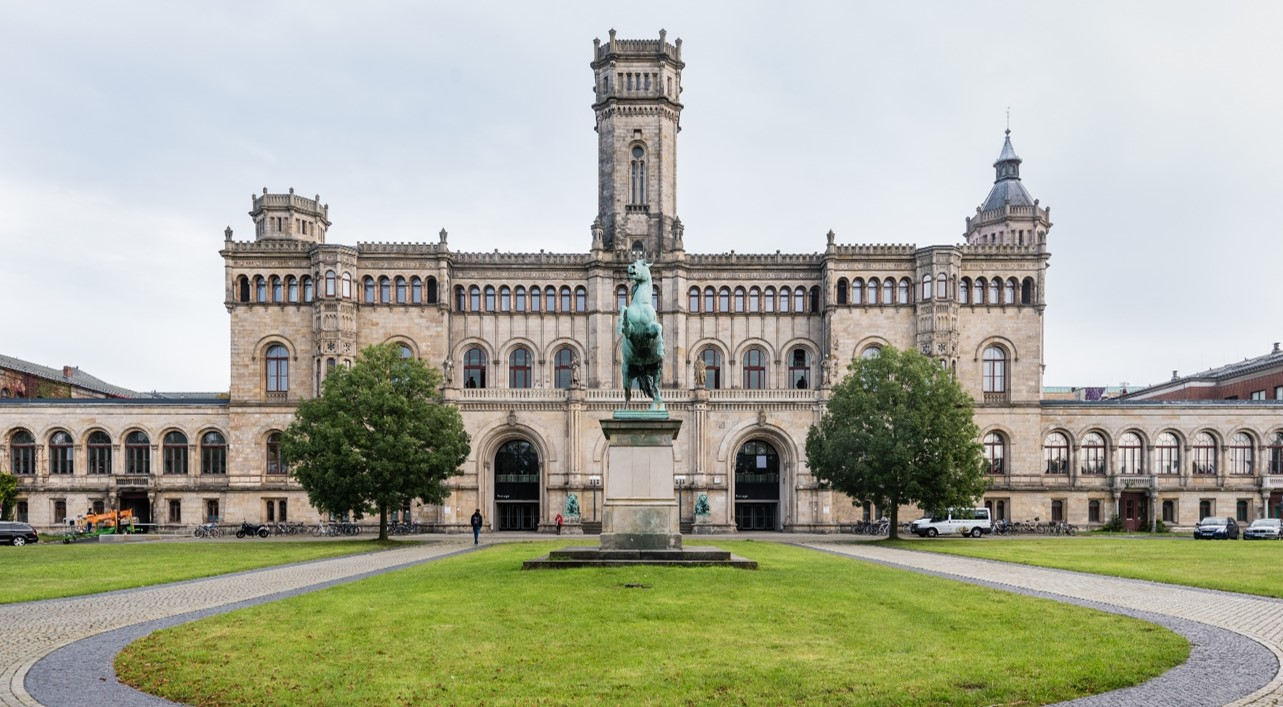
\includegraphics[width=0.65\textwidth]{figures/luh_default_presentation_title_image.jpg}}

% Title page: luhstyle
% \setbeamertemplate{title page}[luhstyle]
% % Add optional title image here
% \addtitlepageimage{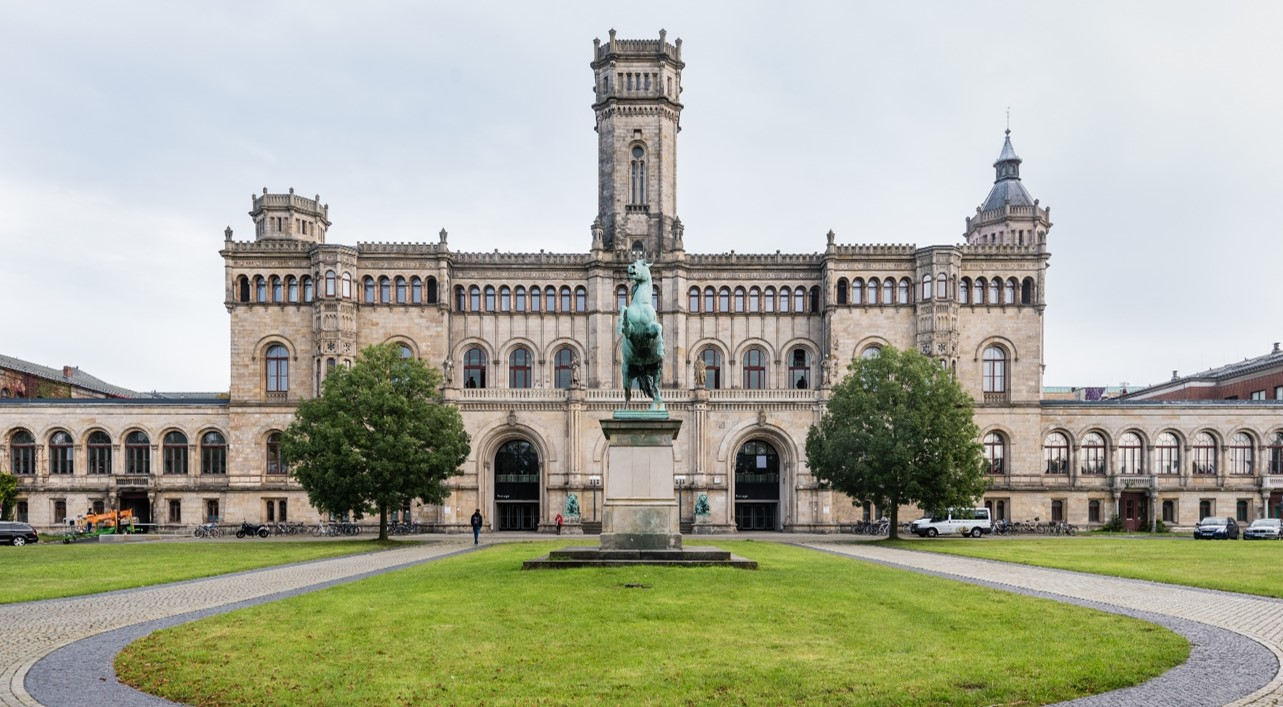
\includegraphics[width=0.75\textwidth]{figures/luh_default_presentation_title_image.jpg}}

\author[Abedjan \& Lindauer]{Ziawasch Abedjan \& Marius Lindauer\\[1em]
	
\includegraphics[height=\logoheight]{../latex_main/figures/luh_logo_rgb_0_80_155.pdf}\qquad
	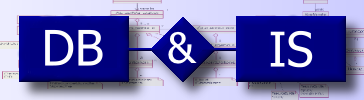
\includegraphics[height=\logoheight]{../latex_main/figures/DBIS_Kurzlogo.png}\qquad

\includegraphics[height=\logoheight]{../latex_main/figures/TNT_darkv4}\qquad

\includegraphics[height=\logoheight]{../latex_main/figures/L3S.jpg}	}
\date{Summer Term 2022; \hspace{0.5em} {
\includegraphics[height=1.5em]{../latex_main/figures/Cc-by-nc-sa_icon.svg.png}}; based on \href{https://ds100.org/fa21/}{[DS100]}
}


%%% Custom Packages
%----------------------------------------------------------------------
% Create dummy content
\usepackage{blindtext}

% Adds a frame with the current page layout. Just call \layout inside of a frame.
\usepackage{layout}


%%% Macros
%\renewcommand{\vec}[1]{\mathbf{#1}}
% \usepackage{bm}
%\let\vecb\bm

\title[Visualization]{DS: Visualization}
\subtitle{Relationships between two quantitative variables}

\graphicspath{ {./figure/} }
%\institute{}


\begin{document}
	
	\maketitle
	\begin{frame}{Scatter plots}
	    \begin{columns}
            \begin{column}{.4\textwidth}
            
            Scatter plots are used to reveal relationships between pairs of numerical variables.
            \begin{itemize}
                \item We often use scatter plots to help inform modeling choices.
                \item For instance, the simple linear model requires the trend in our data to be roughly linear, and for spread to be roughly equal
            \end{itemize}
            
            \end{column}
            
            \begin{column}{.6\textwidth}
            
                       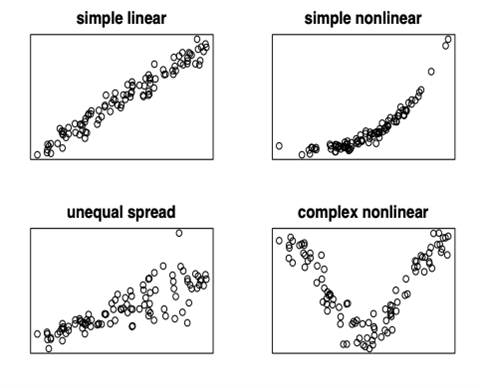
\includegraphics[width=0.8\textwidth]{Bild45}
                       
            \end{column}
        \end{columns}
	\end{frame}
	
	
	\begin{frame}{Scatter plots}
	    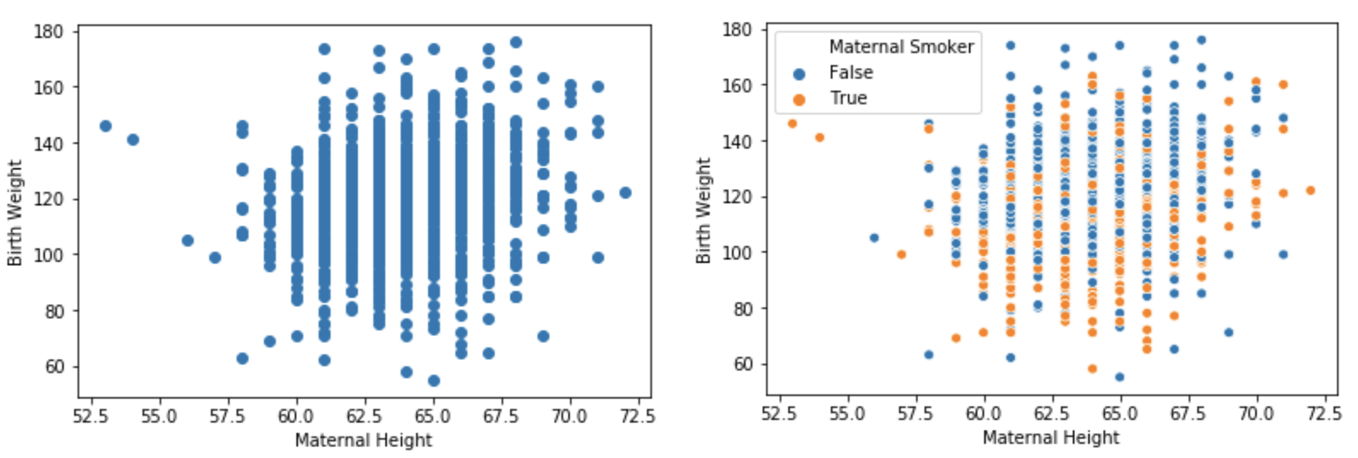
\includegraphics[scale=.35]{Bild46}
	    \begin{itemize}
	        \item We can also use color to encode categorical variables.
	        \item These plots suffer from overplotting – many of the points are on top of one another!
	        \begin{itemize}
	            \item First solution: add a small amount random noise in both the x and y directions. (risky)
	            \item Second solution: use transparency (\texttt{alpha=0.6})
	        \end{itemize}
	    \end{itemize}
	\end{frame}
	
	
	\begin{frame}{Scatter plots}
	    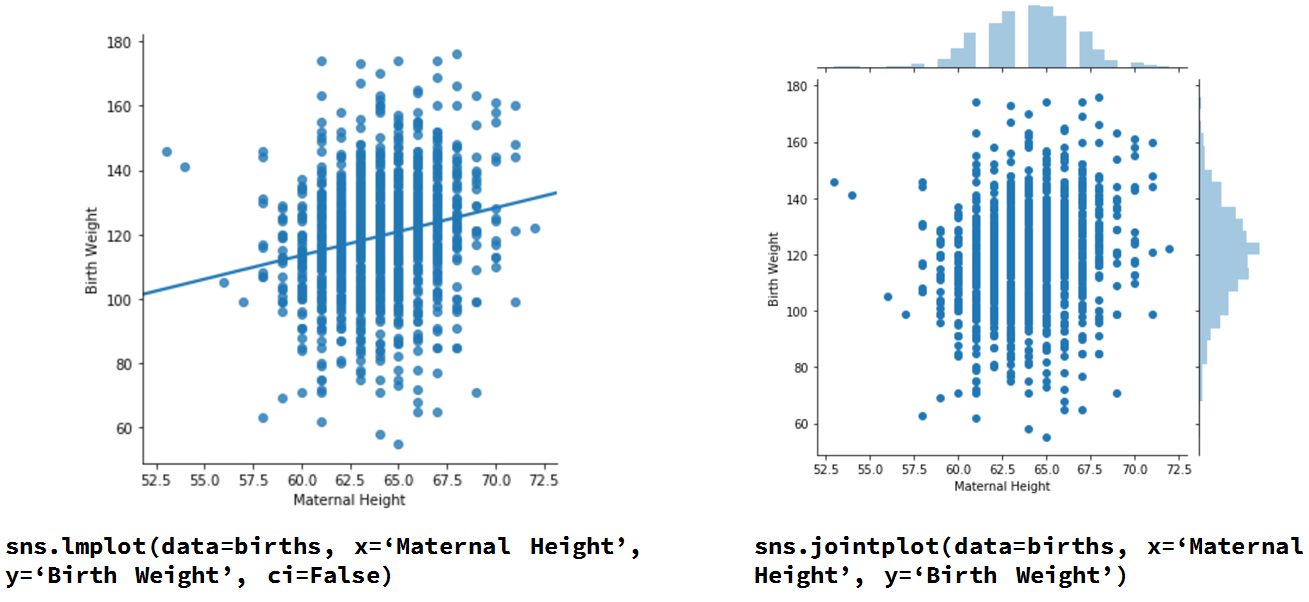
\includegraphics[scale=.4]{Bild47}
	\end{frame}
	
	
	\begin{frame}{Hex plots}
	    \begin{columns}
            \begin{column}{.5\textwidth}
            Can be thought of as a two dimensional histogram. Shows the joint distribution.
            \begin{itemize}
                \item The x-y plane is binned into hexagons
                \item More shaded hexagons typically indicate a greater density/frequency
            \end{itemize}
            
            \bigskip
            Why hexagons instead of squares?
            \begin{itemize}
                \item Easier to see linear relationships
                \item More efficient for covering region
                \item \alert{Visual bias} of squares – drawn to see vertical and horizontal lines
            \end{itemize}
            \end{column}
            
            
            \begin{column}{.5\textwidth}
               \begin{figure}
                       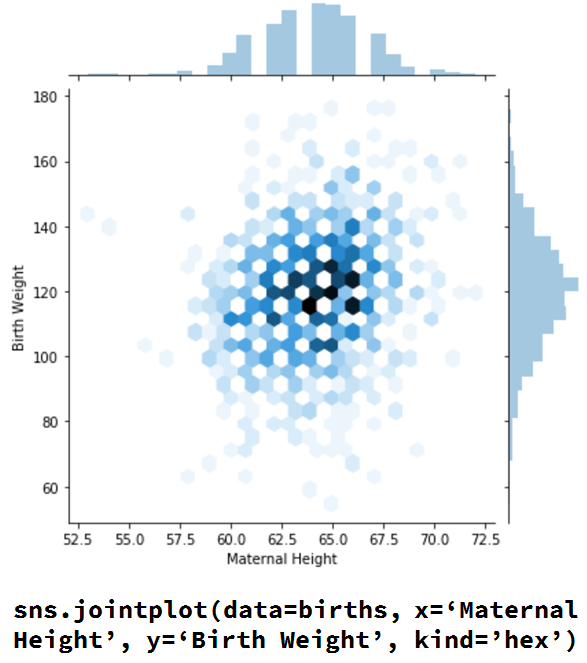
\includegraphics[scale=.33]{Bild48}
                \end{figure}
            \end{column}
        \end{columns}
	\end{frame}
	
	
	
	
	\begin{frame}{Contour plots}
	    \begin{columns}
            \begin{column}{.5\textwidth}
            Contour plots are two dimensional versions of density curves.
            
            \bigskip
            Each of the last few plots has been created by \texttt{sns.jointplot}.
            \begin{itemize}
                \item By default, shows marginal distributions on the horizontal and vertical axes
                \item These are the histograms/density curves of each variable independently.
            \end{itemize}
            \end{column}
            
            
            \begin{column}{.5\textwidth}
               \begin{figure}
                       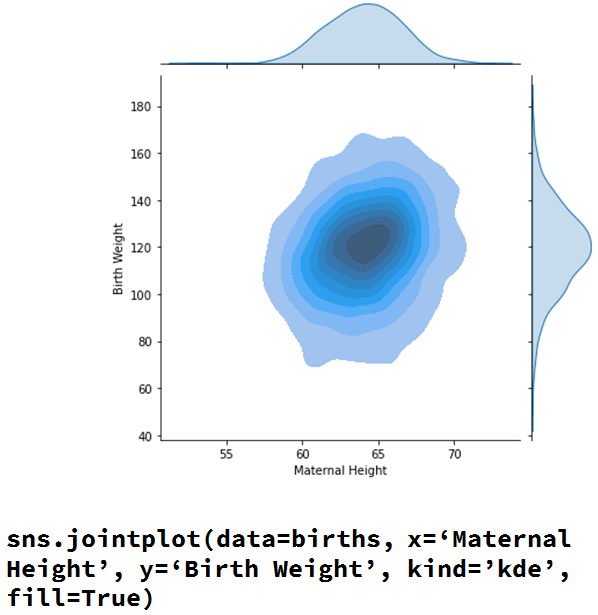
\includegraphics[scale=.35]{Bild49}
                \end{figure}
            \end{column}
        \end{columns}
	\end{frame}
	
	
	\begin{frame}{Intermediate Summary}
	    \begin{itemize}
	        \item Visualization requires a lot of thought!
	        \item Types of variables constrain the charts that you can make.
	        \begin{itemize}
	            \item Single quantitative: rug plot, histogram, density plot, eCDF.
	            \item Two quantitative: scatter plot, hex plot, contour plot.
	            \item Combination: bar plot, overlaid histograms/density plots, SBS box/violin plots.
	        \end{itemize}
	        \item This class primarily uses \texttt{seaborn} and \texttt{matplotlib}.
	        \begin{itemize}
	            \item \texttt{pandas} also has basic built-in plotting methods.
	            \item Many other visualization libraries exist. \texttt{plotly} is one of them.
	            \begin{itemize}
	                \item It very easily creates interactive plots.
	                \item It will appear in lecture code and assignments! 
	            \end{itemize}
	        \end{itemize}
	    \end{itemize}
	\end{frame}
	
	
	
	\begin{frame}{FAIL!}
	    \begin{columns}
            \begin{column}{.5\textwidth}
            \begin{figure}
                       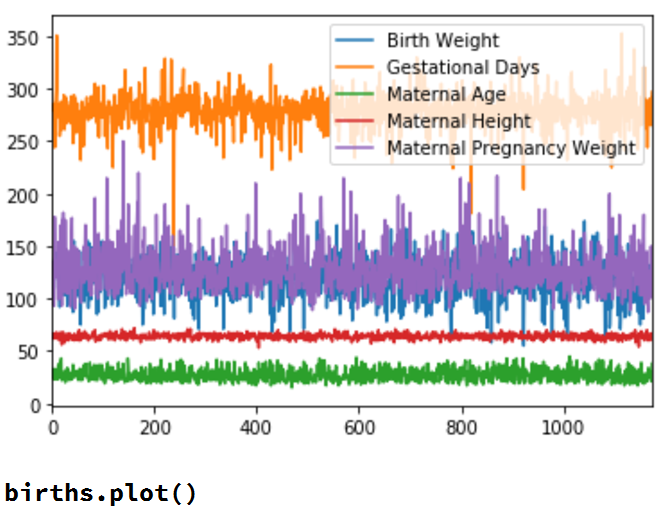
\includegraphics[scale=.35]{Bild50}
                \end{figure}
            \end{column}
            
            
            \begin{column}{.5\textwidth}
                \\
                \bigskip
                \bigskip
               This is the result of calling births.plot(). If you don’t provide any specifications, \texttt{pandas} just guesses what you want visualized. It often makes no sense!

            \end{column}
        \end{columns}
	\end{frame}
	
	
\end{document}